% AICAP 2027 (Aviation Innovation Conference for the Asia-Pacific), NTU Singapore, 27--29 Jan 2027.
% Call for papers: https://event.ntu.edu.sg/AICAP-2027/pages/call-for-papers
%   IEEE double-column format; at most 8 pages including references, appendices and supplementary content;
%   PDF up to 6 MB, submitted through EasyChair; papers due 8 Nov 2026 (time zone not stated).
% Template: Overleaf's official "IEEE Conference Template" (IEEEtran, conference mode).
% Remove every red TODO, and any remaining template text, before submission.
%
% Story, organized after World-in-World (Zhang et al., ICLR 2026) and rewritten for aviation readers:
% - Question: does a world model that predicts well also fly well?
% - Stance, a design choice that does not depend on results: judge a world model by the missions it flies.
% - A ladder of evaluation, each rung closer to flying:
%     rung 0: validation error on the model's own data (World-in-World's "visual quality"); the selection score
%             of Section III-D, set against the layers in Section IV's opening, not a layer of its own;
%     layer 1: prediction error on the plans the planner flies (its "controllability");
%     layer 2: cross-agent counterfactual error (new: physically coupled teams);
%     layer 3: decision quality, scored as the share of costly decisions;
%     layer 4: closed-loop success J.
% - Headline: the pre-registered test of whether layer 2 explains closed-loop differences that layer 1
%   misses (uav_arena/ANALYSIS.md, frozen with tag arena-v0.3). The story must hold whatever the test
%   finds: supported, not established, or the unexpected direction.
% - Each section notes its page budget: 8 pages in all, references included.
\documentclass[conference]{IEEEtran}
\IEEEoverridecommandlockouts
% The preceding line is only needed to identify funding in the first footnote. If that is unneeded, please comment it out.
\usepackage{cite}
\usepackage{amsmath,amssymb,amsfonts}
\usepackage{algorithmic}
\usepackage{graphicx}
\usepackage{array} % ragged-right paragraph columns in Table I
\usepackage{textcomp}
\usepackage{xcolor}
\usepackage{url} % typesets URLs in the bibliography
\usepackage{capt-of} % \captionof, for the teaser under the title
\usepackage{tikz} % Figs. 1 and 4 are drawn in approved_figures_20261105/fig1_teaser.tex and layer_probes.tex, Fig. 3 in figures/decision_timeline.tex
\usetikzlibrary{arrows.meta,decorations.pathreplacing}
\def\BibTeX{{\rm B\kern-.05em{\sc i\kern-.025em b}\kern-.08em
    T\kern-.1667em\lower.7ex\hbox{E}\kern-.125emX}}
\newcommand{\todo}[1]{\textcolor{red}{[TODO: #1]}}
\newcommand{\tbd}{\textcolor{red}{?}} % a result that does not exist yet
% Framed stand-in for a figure that does not exist yet: \figplaceholder{<height>}{<what it will show>}
\newcommand{\figplaceholder}[2]{\fbox{\parbox[c][#1][c]{0.96\linewidth}{\centering\small\todo{#2}}}}

\begin{document}

% Title pattern from World-in-World: a hook, then what the paper does. Avoid a title that presupposes the result.
\title{\todo{Title, e.g.\ Will It Fly? Closed-Loop Evaluation of Learned World Models for Cooperative Slung-Load Transport}
% \thanks{Identify applicable funding agency here. If none, delete this.}
}

\author{\IEEEauthorblockN{\todo{First author}}
\IEEEauthorblockA{\textit{\todo{Department}} \\
\textit{\todo{Organization}}\\
\todo{City, Country} \\
\todo{Email or ORCID}}
\and
\IEEEauthorblockN{\todo{Second author}}
\IEEEauthorblockA{\textit{\todo{Department}} \\
\textit{\todo{Organization}}\\
\todo{City, Country} \\
\todo{Email or ORCID}}
}

% Fig. 1 sits under the title, across both columns, as World-in-World's teaser does. The \twocolumn wrapper is the
% usual IEEEtran way to do that; the inner \renewcommand keeps \maketitle's own \twocolumn from nesting.
\twocolumn[{%
\renewcommand\twocolumn[1][]{#1}%
\maketitle
\begin{center}
% Local proposal only. Original palette and IEEEtran serif typography retained.
% Photo is the existing scene crop; the adjacent coupling diagram is schematic.
\definecolor{jepa}{HTML}{2A78D6}
\definecolor{war}{HTML}{EB6834}
\definecolor{pets}{HTML}{1BAF7A}
\definecolor{refgrey}{HTML}{8A8984}
\definecolor{ink}{HTML}{0B0B0B}
\definecolor{inktwo}{HTML}{52514E}
\definecolor{rule}{HTML}{D3D1C7}
\definecolor{panel}{HTML}{F7F6F3}
\definecolor{banner}{HTML}{ECEBE7}
\definecolor{probe}{HTML}{6250D6}
\begin{tikzpicture}[
  font=\fontsize{8}{9.2}\selectfont, >={Stealth[length=4pt,width=3.5pt]},
  panel/.style={draw=rule,fill=panel,rounded corners=4pt,line width=.5pt},
  heading/.style={font=\fontsize{8}{9.2}\selectfont\bfseries,text=ink,anchor=north west,inner sep=0pt},
  note/.style={font=\fontsize{7.3}{8.5}\selectfont,text=inktwo,inner sep=1pt},
  chip/.style={draw=#1,fill=#1!12,rounded corners=2pt,line width=.6pt,
    text width=3.78cm,font=\fontsize{7}{8.3}\selectfont,align=left,inner xsep=4pt,inner ysep=4pt,anchor=west},
  stage/.style={draw=inktwo,fill=white,rounded corners=2pt,line width=.5pt,
    minimum height=.5cm,text width=3.3cm,align=center,font=\fontsize{8}{9.2}\selectfont\mdseries},
  slot/.style={stage,draw=ink,dash pattern=on 3pt off 1.5pt,line width=.9pt,
    minimum height=.62cm,font=\fontsize{8}{9.2}\selectfont\bfseries},
  flow/.style={->,draw=inktwo,line width=.6pt},
  real/.style={->,draw=ink,line width=.9pt},
  effect/.style={->,draw=probe,line width=.9pt},
  probe/.style={circle,fill=probe,text=white,inner sep=0pt,minimum size=.36cm,font=\tiny\bfseries},
  card/.style={draw=rule,fill=white,rounded corners=3pt,line width=.5pt}
]
\fill[banner,rounded corners=4pt] (0,7.25) rectangle (18,7.85);
\node[font=\small\bfseries,text=ink] at (9,7.55) {Does a model that predicts well also fly well?};

% Replace the predictor; retain the common planner, cost and task.
\draw[panel] (0,2.85) rectangle (4.35,7.05);
\node[heading] at (.15,6.91) {Replace: the predictor};
\node[chip=jepa] at (.15,6.18)
  {JEPA: \texttt{full}, \texttt{no\_cross}, \texttt{flat}\\[2pt]
   Cross-agent information flow};
\node[chip=war] at (.15,5.35) {W-ar: autoregressive state model};
\node[chip=pets] at (.15,4.70) {PETS: probabilistic ensemble};
\node[note,anchor=west] at (.15,4.04) {Physics references};
\node[chip=refgrey] at (.15,3.57)
  {fixed / estimated load mass};

\draw[panel] (4.75,2.85) rectangle (9.6,7.05);
\node[heading,font=\fontsize{7}{8.3}\selectfont\bfseries] at (4.90,6.91) {Keep fixed: MPPI planner and shared cost};
\node[stage] (cand) at (6.90,6.18) {candidate plans};
\node[slot] (wm) at (6.90,5.28) {world model under test};
\node[stage] (fut) at (6.90,4.38) {predicted futures};
\node[stage] (pick) at (6.90,3.48) {cost-weighted plan};
\draw[flow] (cand)--(wm);
\draw[flow] (wm)--(fut);
\draw[flow] (fut)--(pick);
\draw[real] (4.35,5.28)--(wm.west);

% Existing scene plus a schematic of influence transmitted through the load.
\draw[panel] (10.00,2.85) rectangle (18,7.05);
\node[heading] at (10.15,6.91) {Test: shared-load transport};
\draw[card] (10.15,3.05) rectangle (15.05,6.52);
\draw[card] (15.25,3.05) rectangle (17.85,6.52);
\node[heading,font=\fontsize{7.5}{8.5}\selectfont\bfseries] at (10.30,6.37) {Task scene};
\node[heading,font=\fontsize{7.5}{8.5}\selectfont\bfseries] at (15.40,6.37) {Cross-agent effect};
\node[anchor=north west,inner sep=0pt] (scene) at (10.60,5.99)
  {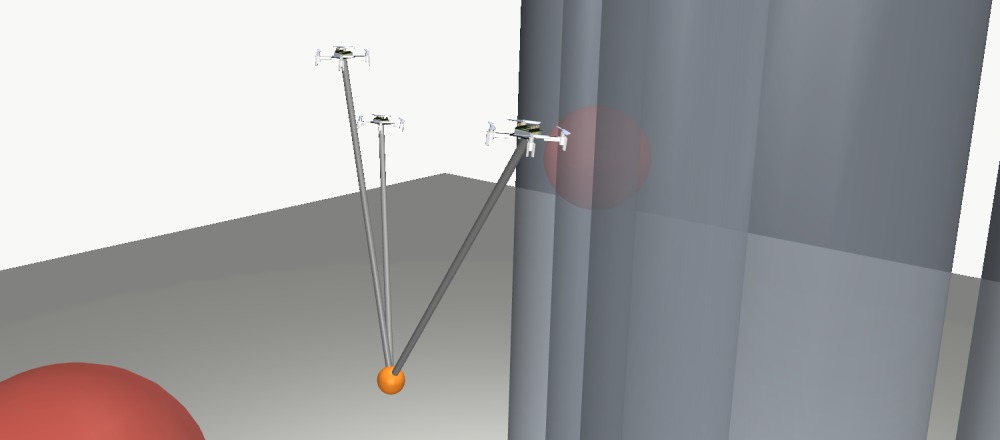
\includegraphics[width=4.00cm]{approved_figures_20261105/teaser_task_crop.png}};
\draw[rule,line width=.5pt] (scene.south west) rectangle (scene.north east);
\node[note,anchor=north west,text width=4.00cm,inner sep=0pt,font=\fontsize{7}{8.3}\selectfont] at (10.60,4.05)
  {Three UAVs carry one load\\[2pt]
   Hidden mass and state delay\\[2pt]
   Static and moving obstacles};
\coordinate (A) at (16.55,5.82);
\coordinate (B) at (15.80,5.30);
\coordinate (C) at (17.25,5.30);
\coordinate (load) at (16.55,4.65);
\foreach \p in {A,B,C} {
  \draw[refgrey,line width=.65pt] (\p)--(load);
  \draw[ink,line width=.7pt] ([xshift=-.15cm]\p)--([xshift=.15cm]\p);
  \draw[ink,line width=.7pt] ([yshift=-.10cm]\p)--([yshift=.10cm]\p);
  \fill[ink] (\p) circle (.045cm);
}
\fill[ink] (load) circle (.085cm);
\node[note,anchor=west] at (16.71,5.82) {A};
\node[note,anchor=east] at (15.64,5.30) {B};
\node[note,anchor=west] at (17.41,5.30) {C};
\node[note,anchor=north] at (16.55,4.46) {load};
\draw[effect] (16.63,5.66)--(16.63,4.87);
\draw[effect] (16.38,4.74)--(15.93,5.13);
\draw[effect] (16.73,4.74)--(17.12,5.13);
\node[note,anchor=north west,text width=2.26cm,inner sep=0pt,font=\fontsize{7}{8.3}\selectfont] at (15.42,4.05)
  {Change A's plan.\\[2pt]
   Predict the response\\[2pt]
   of load and B/C.};

% Real closed loop: state feedback and executed setpoints have distinct paths.
\draw[real] (10.00,6.18)--(cand.east);
\node[note,anchor=south,align=center,font=\fontsize{6}{7}\selectfont] at (9.30,6.23) {delayed\\state};
\draw[real] (pick.east)--(10.00,3.48);
\node[note,anchor=south,align=center,font=\fontsize{6}{7}\selectfont] at (9.30,3.53) {execute\\setpoints};

% Four complementary views, rather than repeating the metric diagrams in Fig.4.
\draw[panel] (0,0) rectangle (18,2.62);
\node[heading] at (.15,2.48) {Measure: from prediction to mission success};
\draw[card,draw=inktwo,line width=.65pt] (10.50,2.12) rectangle (17.85,2.51);
\node[note,font=\fontsize{7}{8}\selectfont] at (14.17,2.315)
  {Oracle U: exact simulator references for layers 1--3};
\foreach \x/\n/\name/\text in {
  .15/1/Prediction/{Same plan, future load},
  4.65/2/Counterfactual/{Changed plan, cross-agent response},
  9.15/3/Decision/{Executed plan, true regret},
  13.65/4/Mission/{Closed-loop flight, success $J$}} {
  \draw[card] (\x,1.11) rectangle ++(4.20,.85);
  \node[probe] at (\x+.28,1.67) {\n};
  \node[anchor=west,font=\fontsize{8}{9.2}\selectfont\bfseries,inner sep=0pt]
    at (\x+.53,1.67) {\name};
  \node[note,anchor=west,font=\fontsize{7}{8}\selectfont,inner sep=0pt]
    at (\x+.15,1.30) {\text};
}
\draw[card,draw=probe,line width=.8pt] (.15,.16) rectangle (17.85,.87);
\node[anchor=west,font=\fontsize{8}{9.2}\selectfont\bfseries,inner sep=0pt,text=ink] at (.32,.51)
  {Pre-registered test};
\node[note,anchor=west,font=\fontsize{8}{9.2}\selectfont,inner sep=0pt] at (3.53,.51)
  {Does cross-agent error $L_2$ add information about success $J$ beyond trajectory error $L_1$?};
\end{tikzpicture}

\captionof{figure}{Testing world models in the loop. A fixed planner flies three quadrotors carrying a slung load in a true simulator; the models under test plug into its world-model slot, and nothing else changes. Layers~1--3, illustrated in Fig.~\ref{fig:probes}, probe the model inside the planner against the true simulator; layer~4 measures closed-loop mission success. The pre-registered test asks whether the cross-agent layer explains success beyond open-loop prediction error.}
\label{fig:loop}
\end{center}
\vspace{2pt}
}]

% Abstract, told the way World-in-World tells its: the question first; the yardstick in use (held-out error)
% set against how a planner uses its model (on the states it visits, to compare plans), which gives the two
% questions the layers ask; and the findings answering them in words. The numbers are in Section V and Fig. 5.
% The IEEE template forbids symbols, special characters, footnotes and math in the title and abstract. IEEE
% convention is 150--250 words. Findings: L1 is the best single guide (rho(L1, J) = -0.88, -0.91 to -0.84); the
% primary test follows the decision rule in uav_arena/ANALYSIS.md, Section 4 (supported: rho(L2, J | L1) = -0.39,
% -0.60 to -0.27); "two of the five model families" is the check outside the plan in Section V (without PETS or
% without flat, the interval contains zero); L3 tracks J least (rho(L3, J) = -0.62, -0.76 to -0.52).
% Held-out error is not claimed to fail across the 30 models: it was not part of the plan.
\begin{abstract}
World models, learned dynamics models, increasingly sit inside the planners of aerial robots, raising a practical question: does a model that predicts well also fly well? The answer is usually assumed: world models are chosen by their error on held-out data, while a planner uses them on the states it visits, to compare plans. When several aircraft carry one slung load, comparing plans means predicting how one aircraft's move propagates through the cables to the load and the other aircraft. We introduce an open-source arena that tests world models in the loop: three Crazyflie~2 quadrotors carry a load of unknown mass past static and moving obstacles, with delayed observations. A ground-truth simulator and one shared planner, in which only the world model changes, score every model on four layers: open-loop prediction, cross-agent counterfactual prediction, decision quality and mission success. Before any test run, we asked of 30 learned world models whether the cross-agent layer explains success differences that open-loop prediction misses. Open-loop error on the planner's states is the best single guide to success; the cross-agent layer explains part of what it misses, mainly through two of five model families; decision quality tracks success least. Physics that estimates the load mass online flies as well as an oracle, and the best learned models about as often as physics with a nominal mass. World models for a team should therefore be validated in the loop, on the plans the planner flies and on how the team responds to one aircraft's move.
\end{abstract}

\begin{IEEEkeywords}
\todo{e.g.\ world models, model-based planning, multi-UAV systems, cable-suspended payload, closed-loop evaluation, benchmark.}
\end{IEEEkeywords}

\section{Introduction}\label{sec:intro}
% Budget, with the abstract: about 1.25 pages including Fig. 1.
% Built like World-in-World's introduction, one move per paragraph: the field and what a world model does;
% the tension and the question; the named gap; what we build; the answer and the stance; the contributions.
% The primary result appears three times: in the abstract, in the last paragraph and in the contributions.

Learned dynamics models are entering the planners and controllers of aerial robots. They capture effects that are hard to model from first principles, such as aerodynamic disturbances~\cite{oconnell2022neuralfly} and the downwash between nearby multirotors~\cite{shi2020neuralswarm,shi2021neuralswarm2}; long-horizon world models have been learned for quadrotor control~\cite{rao2026skyjepa}, and a probabilistic ensemble has guided payload transport by four unmanned aerial vehicles (UAVs) in simulation~\cite{khursheed2024cooperative}. Inside a planner, such a model acts as a world model: given the current state and a candidate plan, it predicts how the vehicles and their load will move, and the planner favors the plans whose predicted futures score best.

% The MLP example is the explore-v1 model on dev (ANALYSIS.md, Section 8): 1.46 cm validation error, 14.6 cm on the
% states the planner visits with exact predictions, 7 of 40 dev missions. Section III-D says in half a sentence
% that explore-v2 was built after it, and that Table II's example MLP was retrained on explore-v2. Min et al.'s
% four predictors span a 12.6-fold range of errors.
In aviation, a controller is not cleared to fly because its model fits data: it is tested in the loop, first in simulation and then with its hardware, before flight tests~\cite{jung2007hil,belcastro2012validation}. Learned world models, by contrast, are usually selected and compared by their open-loop prediction error on held-out data. This is cheap and needs no planner, but held-out data are not the states a planner visits. In our development runs, a multilayer perceptron (MLP) world model erred ten times more on the states the planner visits than on held-out data, and with it the planner completed fewer than one mission in five. The question that matters in flight is a different one: does a model that predicts well also fly well?

Evidence that prediction quality and decision quality can part ways is accumulating. A dynamics model's one-step likelihood need not track the reward its planner achieves~\cite{lambert2020objective}; low prediction error does not guarantee good action choices~\cite{qiu2026adwm,liu2026predictionfidelity}; and in quadrotor simulation, predictors whose errors differ by an order of magnitude reach nearly the same success rate under one planner~\cite{min2026same}. When several aircraft carry one slung load~\cite{lee2014geometric,wahba2024kinodynamic,sun2025agile,lorentz2026crazymarl}, the cables couple them, and a planner that compares candidate plans must predict how one aircraft's move propagates through the cables to the load and to the other aircraft, an effect that the error on a single plan may hide. We therefore measure prediction where the planner uses it and ask two questions. Does a model's error on the plans the planner flies tell whether it flies? And does its error on how one aircraft's move propagates tell more?

We study these questions with an arena that tests world models in the loop (Fig.~\ref{fig:loop}). Three Crazyflie~2 quadrotors carry a cable-suspended load of unknown mass past static and moving obstacles (Fig.~\ref{fig:scene}), with observations delayed by up to 200\,ms. A ground-truth simulator supplies exact references, including the true effect of changing one aircraft's plan. The world models under test all plan with one shared sampling-based planner in which only the world model changes, so differences in flight can be traced to the model. Four evaluation layers then say whether a model flies and where it falls short: open-loop prediction and cross-agent counterfactual prediction, which pose the two questions, then decision quality and closed-loop mission success. The analysis was fixed before any test-set run, so it could not be tuned to the test results.

Across 30 learned world models, open-loop error on the plans the planner flies is the best single guide to mission success, and, as the pre-registered test found, cross-agent counterfactual error explains part of what it misses (Fig.~\ref{fig:scatter}). The evidence comes mainly from one contrast: a probabilistic ensemble predicts the flown plans less accurately than a transformer that encodes the whole team as one token per time step, yet predicts better how one aircraft's move spreads through the team, and flies more often. Decision quality, the layer closest to the mission, tracks success least. A physics model that estimates the load mass online flies as well as an oracle that knows the true state and mass, so the arena measures how close learned models come to physics rather than assuming that they must beat it. A world model for a team, we argue, should be judged by the missions it flies.

Our contributions are threefold:
\begin{itemize}
\item An open-source arena for cooperative slung-load transport with a hidden load mass, observation delay and moving obstacles; a shared planner and predictor interface; and reference rows: an oracle and physics models with a nominal or an online-estimated load mass.
\item A four-layer evaluation that uses the simulator for exact references: open-loop prediction, cross-agent counterfactual prediction, decision quality and closed-loop mission success.
\item A pre-registered test across 30 learned world models, which finds that open-loop error on the planner's states is the best single guide to mission success and that cross-agent counterfactual error explains success beyond it.
\end{itemize}
The code is available at \todo{repository link; an anonymized link if the review is double-blind}.

\section{Related Work}\label{sec:related}
% About half a column. Each paragraph follows the narrative of World-in-World's related work: what the field has
% done, then what our setting adds, stated plainly. World-in-World itself is not cited: only its writing served as a
% model. Claims checked against their sources on 2026-11-03 (workflows wf_e2df83a3-772 and wf_60c00778-c70);
% the EASA sentence rests on Objective SU-01, Issue 02, p. 87. Since 2026-11-05, when Sections III-IV were condensed,
% the second paragraph's last two sentences also carry what Section IV said before: which levels of Yu et al.'s
% ladder the layers reach, and that layer 3 scores the plan the planner would fly, not a ranking of candidates.

\textbf{Assuring learned components in aviation.} Aviation regulators have issued first objectives and a roadmap for assuring machine-learning components~\cite{easa2024concept,faa2024roadmap}. For a learned surrogate model, the European guidance ties the verification of its accuracy to the high-fidelity reference model it approximates~\cite{easa2024concept}. A world model inside a planner acts only through the planner's decisions, so we also test whether its accuracy carries over to them.

\textbf{Decision-aware evaluation of world models.} Decision-level diagnostics score a world model by how it ranks a fixed bank of candidate actions~\cite{qiu2026adwm,liu2026predictionfidelity,rana2026auditing}, and such diagnostics now cover multi-agent world models~\cite{zou2026mawam}. Yu et~al.~\cite{yu2026position} propose a ladder of evaluation levels and a benchmark protocol with exact simulator resets and a fixed optimizer, and ask that lower-level measures be validated against decisions. We run such a protocol, at the ladder's levels of interventional fidelity and planning utility, for aircraft coupled through a shared load. We add a cross-agent counterfactual layer scored against exact ground truth, and score decisions by the plan the planner would fly rather than by how a model ranks candidates.

\textbf{Cooperative slung-load transport.} Methods for teams of multirotors carrying cable-suspended loads include geometric control~\cite{lee2014geometric}, kinodynamic planning~\cite{wahba2024kinodynamic}, learned motor-level policies~\cite{lorentz2026crazymarl} and model-based control that copes with an unknown load mass~\cite{sun2025agile,hajieghrary2026adaptive}. Dynamics models have been compared under one planner for a single quadrotor~\cite{min2026same}, for a single UAV carrying a suspended payload~\cite{belkhale2021meta,jin2025neural} and, in simulation, for a team of four~\cite{khursheed2024cooperative}. We compare 30 learned world models for a team of three quadrotors under one planner.

\section{The Arena}\label{sec:arena}
% Budget: about 1.5 pages including Figs. 2 and 3. Organized like World-in-World's Section 2: what is held fixed, and
% the one thing that varies, the world model. Facts checked on 2026-11-03 against uav_arena's README, PARTICIPANTS,
% TASKS and HARNESS (uav-arena f768261), the W-ar and PETS participant docs, and the JEPA docs on uav/yihao-jepa
% (57e9b1a: all three variants select G6, history 4 and 60,000 steps). Thresholds, cost weights and solver
% settings stay in the released code (paper detail filter). Since 2026-11-04 the prose keeps only the numbers a
% reader needs to follow the story; the settings and the evaluation's parameters are in Table I (tab:arena).
Our arena holds everything but the world model fixed: the aircraft and their onboard control, the missions, the observations and the planner with its cost. This section describes each, then the models under test; Table~\ref{tab:arena} lists the settings.

% The flight is U's evaluated dev episode, re-recorded on 2026-11-03 in the frozen arena-v0.3 checkout (arena venv):
%   PYTHONPATH=. python -m uav_arena.replay record --participant oracle --seed 0 --condition static+moving/100ms \
%     --workers 7 --out data/uav_arena/replays/oracle_s0_moving100_arena-v0.3.npz
% Success at 8.5 s with the load 0.010071 m from the goal, as in the dev results (oracle_mppi_dev_s0-5_v3.json).
% The earlier oracle_s0_moving100.npz (2026-10-26) predates per-episode solver reseeding (eda1e43) and flew another
% path (9.5 s). figures/src/extract_topview.py (arena venv) dumps the paths, pillars and moving spheres, taking each
% sphere's segment ends from the scenario (Mover.a, Mover.b); figures/src/plot_topview.py (matplotlib) draws them,
% with two insets. Top left, figures/src/arena_team_closeup.jpg (render_scene.py at 3.8 s: azimuth 230, elevation
% -60, distance 1.3, team-centred, --path-colors 2a78d6,199e70,c98500,0b0b0b --paint-load --mover-color e34948
% --opaque-pillars --no-paths --color-cables --cable-width 0.008; rows 185-650 and columns 150-1240 of the
% 1600 x 1000 output, which leave out two pillars passing close to the camera); sphere 0 is 0.53 m from the nearest
% aircraft. Bottom left, figures/src/arena_team_pillar.jpg (the same options plus --hide-goal, at 6.4 s: azimuth 80,
% elevation -35, distance 1.3; rows 250-850 and columns 40-1300), so that a pillar is in view as well; the goal
% marker is hidden because a cable crosses it in the picture. Until 2026-11-05 the inset showed 2.2 s, when the team
% passes 0.2 m from two pillars: from every angle a pillar sat right behind or in front of it, and the arena's
% translucent pillars let a sphere behind one show through. A search over times and cameras (segmentation renders,
% no multisampling) found the top-left view as the one that shows the team and a sphere whole and apart with no
% pillar beside either; paths are left out because the aircraft's recent path crosses the sphere in the picture.
% About 2.4 in tall at column width. The view stops at |y| = 1.45 m; the workspace reaches 2.5 m. Each moving
% sphere shuttles along one straight, slanted segment; its sweep is drawn as a capsule of radius 0.15 m along it.
% The spheres do not collide with pillars, and two segments cross one (sphere 0 pillar 1, sphere 1 pillar 3); the
% top view draws the pillars opaque over the sweeps, as a view from above would show them. Aircraft colors and the
% validator result are in plot_topview.py's docstring.
\begin{figure}[t]
\centering
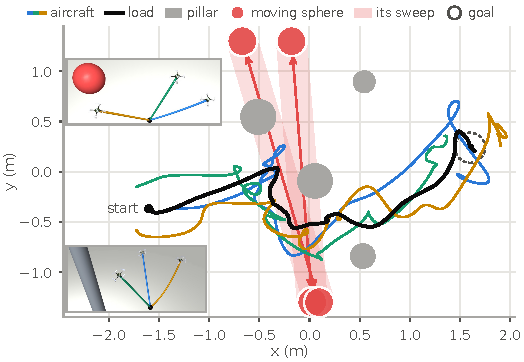
\includegraphics[width=\linewidth]{figures/arena_topview.pdf}
\caption{Top view of one flight of the oracle U (development layout~0, moving spheres, 100\,ms delay), from the start to the goal: the paths of the three aircraft, one color each, and of the load, the four pillars and the two moving spheres. Each sphere is drawn at both ends of the straight segment it shuttles along, with the strip it sweeps. Insets: the team at 3.8\,s seen from above, with a moving sphere 0.5\,m away (top), and at 6.4\,s, with a pillar behind it (bottom); each cable is drawn in its aircraft's color.}
\label{fig:scene}
\end{figure}

% The settings that left the prose on 2026-11-04, each checked on 2026-11-03 (wf_0905a814-d2b) against uav_arena's
% README, PARTICIPANTS, TASKS and HARNESS (uav-arena f768261), ANALYSIS.md (arena-v0.3) and the participant docs.
% The layer-2 scale is from HARNESS.md, Section 4 (U's dev states, A changes); the cost unit from ANALYSIS.md,
% Section 3; the power from ANALYSIS.md, Section 4.
% Local review only. Replace the original table block only after approval.
\begin{table}[t]
\caption{Task, Planning, and Evaluation Settings}
\label{tab:arena}
\centering
\footnotesize
\setlength{\tabcolsep}{3pt}
\renewcommand{\arraystretch}{1.12}
\begin{tabular}{@{}>{\raggedright\arraybackslash}p{0.245\columnwidth}>{\raggedright\arraybackslash}p{\dimexpr0.755\columnwidth-6pt\relax}@{}}
\hline
\multicolumn{2}{@{}l}{\textbf{Task and environment}} \\
\hline
Team & Three Crazyflie~2 quadrotors; one load; 0.6\,m tension-only cables \\
Load mass & 10--40\,g per layout, hidden; nominal mass 25\,g \\
Obstacles & Four pillars, with or without two moving spheres (0.25--0.45\,m/s) \\
Mission & Goal 3.2\,m ahead; time limit 20\,s \\
Success criterion & Load within 0.15\,m of the goal, below 0.2\,m/s, continuously for 0.5\,s \\
\hline
\multicolumn{2}{@{}l}{\textbf{Control and planning}} \\
\hline
Simulation/control & MuJoCo and onboard Lee controllers, both at 500\,Hz \\
Decision rate & 10\,Hz \\
Observation delay & 0, 50, 100, or 200\,ms \\
Shared planner & MPPI; 512 candidate plans per decision \\
Planning horizon & 15 decisions (1.5\,s) \\
Setpoint moves & At most 0.12\,m per axis \\
\hline
\multicolumn{2}{@{}l}{\textbf{Data and evaluation}} \\
\hline
Training budgets & 500 / 2,000 episodes; 500 uses the first quarter of the same dataset \\
Full training set & 170,304 decisions (4.7\,h); 100 separate validation episodes \\
Main model set & 5 model rows $\times$ 2 budgets $\times$ 3 new seeds $=$ 30 models; 1.28--1.37\,M parameters \\
Test coverage & 50 layouts $\times$ 2 obstacle settings $\times$ 4 delays $=$ 400 episodes per model \\
Probe states & Every fifth decision of U's test flights; 8,660 states in total \\
Uncertainty & 95\% intervals; 10,000 bootstrap resamples of the 50 test layouts \\
\hline
\end{tabular}
\end{table}

\subsection{Task and Plant}
Cooperative slung-load transport couples the aircraft through the cables: when one aircraft changes course, the load swings and the other two aircraft feel the pull. Predicting that propagation is what layer~2 probes (Section~\ref{sec:layers}). Three further features make prediction matter: the load mass is unknown, observations arrive late and obstacles move.

Three Crazyflie~2 quadrotors, with airframes from MuJoCo Menagerie~\cite{todorov2012mujoco,menagerie2022github}, carry one load on tension-only cables. Each aircraft flies with the geometric tracking controller of the Crazyflie firmware~\cite{imrclab2024firmware}, based on Lee et~al.~\cite{lee2010geometric} and compiled unchanged, so a planner commands setpoints rather than thrusts. The load mass changes from layout to layout and is hidden from every decision maker except the oracle (Section~\ref{sec:planner}), so the same setpoints move the team differently from one layout to the next.

A mission starts from a settled hover and succeeds once the load settles at a goal past four pillars and, in half of the conditions, two spheres that shuttle across the path (Fig.~\ref{fig:scene}). It fails when an aircraft, the load or a cable touches an obstacle, when two aircraft collide, when an aircraft or the load hits the floor, when the team leaves the workspace, or when time runs out.

% Fig. 3 carries what a decision maker observes and never observes, the setpoints that bridge the delay, the
% plan horizon and the onboard loop (moved out of the prose on 2026-11-04); the prose keeps why the delay matters.
% Since 2026-11-06 the original figures/decision_timeline.tex (121 pt tall) again, not the reviewed version in
% approved_figures_20261105 (206 pt): both carry the same information, and the shorter one keeps the paper at 8 pages.
\begin{figure}[t]
\centering
% Fig. 3, one decision of the shared planner in time (Sections III-B and III-C): the delayed state, the setpoints
% sent since, the plan, the onboard loop, and what is and is not observed. Every row of the shared planner but the
% oracle U plans this way; U starts from the true current state. Drawn at column width in the vocabulary of Fig. 1
% (figures/fig1_teaser.tex). Facts from Section III and Table I: decisions at 10 Hz on a state up to 200 ms
% old; plans of 15 decisions (1.5 s); Lee controllers at 500 Hz on the true state; a setpoint slides to its new
% value (ramps) over one decision period. The time axis is to scale, with the delay drawn at 200 ms. The
% aircraft states include attitudes and rotation rates; the load's and the spheres' are positions and velocities.
\definecolor{ink}{HTML}{0B0B0B}
\definecolor{inktwo}{HTML}{52514E}
\definecolor{rule}{HTML}{D3D1C7}
\definecolor{panel}{HTML}{F7F6F3}
\definecolor{refgrey}{HTML}{8A8984}
\begin{tikzpicture}[
  font=\scriptsize, >={Stealth[length=3.5pt,width=3pt]},
  heading/.style={font=\scriptsize\bfseries, text=ink, anchor=west, inner sep=0pt},
  note/.style={font=\scriptsize, text=inktwo, inner sep=0pt, align=left},
  brace/.style={decorate, decoration={brace, amplitude=2.5pt}, draw=inktwo, line width=0.5pt},
]
\def\now{2.9}   % the decision at t
\def\dt{0.34}   % one decision period, 0.1 s
% The planner's clock: earlier observations, the delayed state, the decision and one candidate plan.
\node[heading] at (0,2.75) {Planner, 10\,Hz};
\draw[->, inktwo, line width=0.6pt] (0,2.0) -- (8.8,2.0);
\node[note, anchor=south east] at (8.8,2.06) {time};
\foreach \k in {-8,...,15} \draw[inktwo, line width=0.45pt] ({\now+\dt*\k},1.94) -- ({\now+\dt*\k},2.06);
\foreach \k in {-8,...,-3} \fill[refgrey] ({\now+\dt*\k},2.0) circle (1.5pt);
\fill[ink] ({\now-2*\dt},2.0) circle (2pt);
\node[note, anchor=south] at ({\now-5.5*\dt},2.1) {history};
\node[note, anchor=north east, text=ink] at ({\now-2*\dt-0.14},1.92) {state at $t-d$};
\draw[brace] ({\now-2*\dt},2.2) -- (\now,2.2) node[midway, above=2.5pt, note] {$d$};
\draw[brace] (\now,2.2) -- ({\now+15*\dt},2.2)
  node[midway, above=2.5pt, note, text=ink] {a candidate plan: 15 decisions, 1.5\,s};
\draw[ink, line width=0.9pt] (\now,1.72) -- (\now,2.62) node[above=1pt, note, text=ink] {decision at $t$};
% The setpoints sent since t - d, which a model replays to bridge the delay.
\foreach \k in {-2,-1} \draw[->, ink, line width=0.6pt] ({\now+\dt*\k},1.62) -- ({\now+\dt*\k},1.9);
\node[note, anchor=north, align=center, text=ink] at ({\now-1.5*\dt},1.58) {setpoints sent\\since $t-d$};
\node[note, anchor=north west, text width=5.45cm] at ({\now+0.35},1.88)
  {the world model predicts the aircraft positions and the load's position and velocity at each decision};
% The onboard loop, and what is and is not observed.
\fill[panel] (0,0.72) rectangle (8.8,1.1);
\foreach \i in {0,...,125} \draw[rule, line width=0.3pt] ({0.07*\i},0.76) -- ({0.07*\i},1.06);
\node[note, text=ink, fill=panel, inner xsep=2pt, inner ysep=1pt] at (4.4,0.91)
  {\textbf{Onboard, 500\,Hz:} Lee controllers on the true state; setpoints ramp over 0.1\,s};
\node[note, anchor=north west] at (0,0.6)
  {\textit{Observed:} goal, pillars, setpoints sent; from $t-d$, the aircraft, load and sphere states.\\
   \textit{Never observed:} load mass, cable tensions, controller and motor states.};
\end{tikzpicture}

\caption{One decision of the shared planner, in time, as every row but the oracle U sees it.}
\label{fig:decision}
\end{figure}

\subsection{Information and Latency}
Decisions are made ten times a second on a state up to 200\,ms old, while the onboard controllers act on the true current state (Fig.~\ref{fig:decision}). A world model must therefore also predict how the team moved during the delay, from the setpoints sent since. Observations are states rather than images: this isolates the prediction of dynamics, which the layers score, from perception, which we leave to future work (Section~\ref{sec:discussion}).

Two obstacle settings, the pillars alone or with the moving spheres, crossed with four delays give eight conditions. A layout keeps its pillars and load mass in all eight and its sphere motions at every delay, so conditions are compared on the same layouts; the test layouts give 400 test episodes. Training, validation, development and test layouts are disjoint.

\subsection{Shared Planner and Predictor Interface}\label{sec:planner}
The reference rows and the learned world models all plan with the same model predictive path integral (MPPI) planner~\cite{williams2017mppi}, as implemented in stable-worldmodel~\cite{maes2026stableworldmodel}, with the same actions and cost; only the predictor changes. At each decision, MPPI samples candidate plans for the next 1.5\,s, has the predictor roll each one out, and commands a cost-weighted average of them (Fig.~\ref{fig:loop}).

The predictor bridges the delay itself, may keep a history of the episode's earlier observations, and returns for each candidate what the cost reads (Fig.~\ref{fig:decision}). The cost charges the load's distance from the goal, its speed near the goal and the size of the moves, and penalizes predicted violations of safety margins: clearance from the obstacles for aircraft, load and cables, separation between the aircraft, and the heights of the load above the floor and of each aircraft above the load. For every row alike, the spheres' future positions are extrapolated from their observed velocity, and on a given layout MPPI draws the same random samples.

With the true simulator as its predictor, the planner becomes the oracle~U: it starts every rollout from the true, undelayed state, with the true load mass and the onboard states, so its predictions are exact. This privilege makes U the answer key for layers~1--3.

\subsection{Models Under Test}\label{sec:rows}
\textbf{Reference rows.} Two physics rows set the scale for the learned models. They run U's simulator without its privilege: from the delayed observation, they carry the unobserved controller and motor states in a copy of the known onboard flight stack and bridge the delay by replaying the setpoints already sent, as a Smith predictor does; with the true mass, they reproduce U's predictions. Nominal physics assumes a fixed load mass; physics with online mass estimation keeps 16 models on a 2\,g grid and plans with the one that best predicted the preceding 0.5\,s of observations.

\textbf{Learned world models.} The learned models differ in how they represent the team. The entity-token JEPA (joint-embedding predictive architecture) follows LeWorldModel~\cite{maes2026leworldmodel}. It encodes recent observations as one token per aircraft and one for the load and, conditioned on each aircraft's setpoints, predicts future tokens in latent space; a readout, trained jointly, decodes them into the positions and velocities the cost reads. Its three variants differ only in how information flows between entities, so they vary the cross-agent structure that layer~2 probes. In \texttt{full}, every token attends to every token; in \texttt{no\_cross}, aircraft tokens do not attend to other aircraft, so information between aircraft passes only through the load token; \texttt{flat} merges each frame into one token. W-ar, an autoregressive state model, uses the \texttt{full} backbone but predicts state changes directly, step by step, without latent targets. PETS (probabilistic ensembles with trajectory sampling)~\cite{chua2018pets} is an ensemble of probabilistic networks, the model that has guided four-UAV transport in simulation~\cite{khursheed2024cooperative}. Because the planner takes one trajectory per candidate, each candidate follows the mean of one randomly drawn member rather than the sampled particles of published PETS.

% The MLP of the introduction is the example participant trained on explore-v1 (7 of 40 dev missions);
% retrained on explore-v2 it flies 21 of 40 and is Table II's example row (TASKS.md, "Example participant").
% Data: explore-v2, obstacle-free. Policies: CrazyMARL commands rotor thrusts at 250 Hz; TD-MPC2 ran its defaults
% with its options for tasks that terminate, DreamerV3 its dmc_proprio preset (world model 0.54 M parameters).
\textbf{Data and training.} The training and validation data come from a behavior policy that flies the team in formation between random waypoints, without obstacles, and perturbs each aircraft's moves at MPPI's sampling scale (Table~\ref{tab:arena}), so that they cover the moves the planner commands. The data behind the MLP of Section~\ref{sec:intro} did not; retrained on these, that MLP is the example row of Table~\ref{tab:results}, outside the 30. For each of the five learned rows, at most eight configurations were compared by validation error alone, the load position error on held-out episodes, and the chosen one was trained with three new seeds on all 2,000 training episodes and on the first 500. Within each model row, both budgets use the same configuration and number of optimization steps. This gives 30 learned world models of similar size (Table~\ref{tab:arena}).

\textbf{Policies without the shared planner.} Three policies show how far published methods get without the shared planner; each was trained with its official code on arena layouts, with three seeds (Table~\ref{tab:arena}). CrazyMARL~\cite{lorentz2026crazymarl} commands rotor thrusts from each aircraft's fresh own state and delayed observations of the rest; it was retrained for its official budget of $2\times10^9$ steps per seed, with 8,192 parallel environments (half the official 16,384), in its own simulator, configured with the arena's airframes, cables, obstacles and delays and the nominal load mass. TD-MPC2~\cite{hansen2024tdmpc2} and DreamerV3~\cite{hafner2023dreamerv3} trained online for $2\times10^6$ steps per seed from the delayed observation with the state-based settings of their official code, on about twelve times the world models' data, with a reward for the load's progress, a bonus on success and a penalty on failure. The policies do not implement the predictor interface that layers~1--3 call, so they are scored on layer~4 only.


\section{Evaluation Layers}\label{sec:layers}
% Budget: about 1 page including Fig. 4. Narrated after World-in-World's Section 2: a short design overview with
% the questions, which Fig. 4 draws together with layers 1-3 (the procedure left the prose on 2026-11-04); then
% one paragraph per layer in a fixed order: what it asks, why it matters, how it is scored. World-in-World leaves
% its metrics to captions and an appendix; our layers are a contribution, so they are defined here. Layer names,
% used throughout: open-loop prediction, cross-agent counterfactual prediction, decision quality, mission success
% (the cards of Figs. 1 and 4: Prediction, Counterfactual, Decision, Mission).
% Definitions: uav_arena/ANALYSIS.md (frozen with arena-v0.3) and HARNESS.md (uav-arena f768261); the layer-2 scale
% from HARNESS.md, Section 4 (U's dev states, A changes); the cost unit from ANALYSIS.md, Section 3. Layer 3's
% reliable-reference rule is stated in the text since the fact-check of 2026-11-03 (wf_0905a814-d2b): Table II's L3
% needs it (physics + mass est. 3.7% on the reliable questions, 5.3% on all). Left to the released code (paper detail
% filter): layer 2's fixed-offset changes and the changed aircraft's own error, and the repeats and common random
% numbers for stochastic predictors. Secondary diagnostics (validation score, top-k regret, ranking metrics, the
% parts of L2) enter Section V where a finding uses them. Yu et al.'s ladder (arXiv 2606.15032v2, Table 7): L1 is
% logged-future prediction (our validation error), L4 interventional fidelity (layers 1-2), L7 planning utility
% (layers 3-4); since 2026-11-05 Section II states this. Also left the text on 2026-11-05: U scores exactly zero on
% layers 1-3 (Table II), which checks that the questions and their answers are rebuilt exactly; "being closer by
% design need not mean tracking success more closely" (Section V shows it); and, for layer 3, that off-policy
% evaluation scores a method by the regret of the policies it selects (fu2021dope, no longer cited).
\begin{figure}[t]
\centering
% Focused revision: same original palette and serif font; schematic, not experimental data.
% Fig. 4, how layers 1-3 pose and score a question (Section IV): the question and its two answers on top, then
% one panel per layer, numbered and named as the probes and cards of Fig. 1 (figures/fig1_teaser.tex), in the
% same vocabulary: solid ink for the truth, dashed violet for the model. A sketch, not data: the paths, arrows
% and costs are illustrative. Definitions from uav_arena/ANALYSIS.md and HARNESS.md, as in Section IV.
\definecolor{ink}{HTML}{0B0B0B}
\definecolor{inktwo}{HTML}{52514E}
\definecolor{rule}{HTML}{D3D1C7}
\definecolor{panel}{HTML}{F7F6F3}
\definecolor{refgrey}{HTML}{8A8984}
\definecolor{probe}{HTML}{6250D6}
\begin{tikzpicture}[
  font=\fontsize{7.5}{8.6}\selectfont, >={Stealth[length=3.5pt,width=3pt]},
  panel/.style={draw=rule, fill=panel, rounded corners=3pt, line width=0.5pt},
  box/.style={draw=inktwo, fill=white, rounded corners=2pt, line width=0.5pt, align=left, inner xsep=3pt,
    inner ysep=2.5pt, text width=6.20cm},
  slot/.style={draw=ink, dash pattern=on 2.5pt off 1.2pt, fill=white, rounded corners=2pt, line width=0.8pt,
    align=left, inner xsep=3pt, inner ysep=2.5pt, text width=6.20cm},
  probe/.style={circle, fill=probe, text=white, inner sep=0pt, minimum size=0.32cm, font=\tiny\bfseries},
  flow/.style={->, draw=inktwo, line width=0.6pt},
  truth/.style={draw=ink, line width=0.8pt},
  pred/.style={draw=probe, line width=0.8pt, dash pattern=on 2pt off 1pt},
  heading/.style={font=\fontsize{7.5}{8.6}\selectfont\bfseries, text=ink, anchor=west, inner sep=0pt},
  note/.style={font=\fontsize{7.2}{8.2}\selectfont, text=inktwo, inner sep=0pt, align=left},
  craft/.style={circle, fill=inktwo, inner sep=0pt, minimum size=3.4pt},
  load/.style={circle, fill=ink, inner sep=0pt, minimum size=4.6pt},
  ring/.style={circle, draw=probe, fill=white, line width=0.9pt, inner sep=0pt, minimum size=5pt},
]
% Top: a question, a state from U's flight, answered by the true simulator and by the model.
\draw[panel] (0,3.27) rectangle (8.8,4.59);
\node[heading] at (0.12,4.42) {A question: a state U planned from in a test flight};
\draw[inktwo, line width=0.6pt] (0.2,3.39) .. controls (0.6,4.12) and (1.05,3.32) .. (1.75,4.12)
  node[pos=0.12, craft]{} node[pos=0.37, craft]{} node[pos=0.86, craft]{}
  node[pos=0.62, ring](q){};
\node[box, anchor=west] (sim) at (2.1,4.03) {\textbf{True simulator}: exact reset and rollout};
\node[slot, anchor=west] (mod) at (2.1,3.51) {\textbf{Model}: prediction from the delayed observation};
\draw[flow] (q) to[out=40, in=180] (sim.west);
\draw[flow] (q) to[out=-40, in=180] (mod.west);
% Bottom: one panel per layer.
\foreach \x/\n/\name in {0/1/Prediction, 2.975/2/Counterfactual, 5.95/3/Decision} {
  \draw[panel] (\x,-0.22) rectangle ++(2.85,3.37);
  \node[probe] at (\x+0.27,2.90) {\n};
  \node[heading] at (\x+0.5,2.90) {\name};
}
% 1: U's plan, the load's predicted and true paths.
\begin{scope}[yshift=0cm]
  \draw[truth] (0.3,1.32) .. controls (1.0,1.42) and (1.8,2.2) .. (2.55,2.42)
    coordinate[pos=0.4](t1) coordinate[pos=0.7](t2) coordinate[pos=1](t3);
  \draw[pred] (0.3,1.32) .. controls (1.0,1.37) and (1.8,1.75) .. (2.55,1.85)
    coordinate[pos=0.4](p1) coordinate[pos=0.7](p2) coordinate[pos=1](p3);
  \foreach \i in {1,2,3} \draw[probe!45, line width=0.6pt] (t\i) -- (p\i);
  \node[load] at (0.3,1.32) {};
  \node[note, anchor=south east] at (2.6,2.46) {true};
  \node[note, anchor=north, text=probe] at (1.95,1.6) {model};
  \node[note, anchor=north west, text width=2.62cm] at (0.12,0.86)
    {Same plan $a$; load only.\\[3pt]$L_1$: mean position error};
\end{scope}
% 2: one aircraft's plan nudged, the predicted and true effects on the load and the other two aircraft.
\begin{scope}[shift={(2.975,0)}]
  \coordinate (a1) at (0.8,2.15); \coordinate (a2) at (1.55,2.27); \coordinate (a3) at (2.3,2.15);
  \coordinate (l) at (1.55,1.5);
  \foreach \a in {a1,a2,a3} \draw[rule, line width=0.6pt] (\a) -- (l);
  \draw[->, ink, line width=0.7pt] (a1) -- ++(0,0.3);
  \node[note, anchor=west, text=ink] at (0.12,2.65) {A: $a\to a'$};
  \node[note, anchor=south] at (1.55,2.47) {B};
  \node[note, anchor=west] at (2.35,2.15) {C};
  \draw[->, truth] (l) -- ++(-0.45,-0.14) node[note, anchor=north east, text=ink] {$\Delta x$};
  \draw[->, pred] (l) -- ++(-0.55,0.08) node[note, anchor=east, text=probe] {$\Delta\hat{x}$};
  \draw[->, ink, line width=0.6pt] (a2) -- ++(-0.27,0.05);
  \draw[->, pred, line width=0.6pt] (a2) -- ++(-0.2,0.14);
  \draw[->, ink, line width=0.6pt] (a3) -- ++(-0.25,0.0);
  \draw[->, pred, line width=0.6pt] (a3) -- ++(-0.3,-0.12);
  \foreach \a in {a1,a2,a3} \node[craft] at (\a) {};
  \node[load] at (l) {};
  \node[note, anchor=west] at (1.73,1.5) {load};
  \node[note, anchor=north west, text width=2.62cm] at (0.12,0.86)
    {Change A only.\\Score load and B/C.\\[3pt]$L_2$: effect error};
\end{scope}
% 3: the weighted execution plan, placed by its true cost.
\begin{scope}[shift={(5.95,0)}]
  \fill[probe!9] (1.3,1.3) rectangle (2.65,2.32);
  \draw[probe, dash pattern=on 1.5pt off 1pt, line width=0.5pt] (1.3,1.3) -- (1.3,2.32);
  \node[note, anchor=north east, text=probe] at (2.62,2.29) {costly};
  \draw[->, inktwo, line width=0.5pt] (0.2,1.28) -- (2.7,1.28);
  \node[note, anchor=north east] at (2.7,1.24) {true cost};
  \node[note, anchor=north, text=probe] at (1.3,1.24) {$+1$ unit};
  \foreach \x in {0.38,0.55,0.74,0.93,1.12,1.48,1.7,1.95,2.2,2.45} \fill[refgrey] (\x,1.41) circle (1.1pt);
  \node[load] at (0.62,1.72) {};
  \node[ring] at (2.05,1.72) {};
  \draw[<->, inktwo, line width=0.5pt] (0.7,1.9) -- (1.97,1.9);
  \node[note, anchor=south] at (0.9,1.91) {regret};
  \node[note, anchor=east] at (0.53,1.72) {U};
  \node[note, anchor=west, text=probe, font=\fontsize{6.5}{7.5}\selectfont] at (2.22,1.72) {model};
  \node[note, anchor=north west, text width=2.62cm] at (0.12,0.86)
    {Weighted execution plan.\\[3pt]$L_3$: costly-plan rate\\(regret $>1$)};
\end{scope}

% Independent top-level nodes avoid renderer-dependent shifts in inline fractions.
\node[note,anchor=base west,font=\fontsize{6.8}{7.8}\selectfont] at (0.12,-0.50) {$L_2$:};
\foreach \cx in {0.70,1.65} {
  \node[anchor=center,inner sep=0pt,font=\fontsize{5}{5}\selectfont] at (\cx,-0.35) {1};
  \draw[inktwo,line width=0.3pt] (\cx-0.055,-0.46)--(\cx+0.055,-0.46);
  \node[anchor=center,inner sep=0pt,font=\fontsize{5}{5}\selectfont] at (\cx,-0.57) {2};
}
\node[note,anchor=base west,font=\fontsize{6.8}{7.8}\selectfont] at (0.85,-0.50) {load +};
\node[note,anchor=base west,font=\fontsize{6.8}{7.8}\selectfont] at (1.80,-0.50) {mean(B,C); repeat for each source UAV.};
\end{tikzpicture}

\caption{How layers~1--3 score a world model. Solid: true; dashed: the model's prediction; grey dots: the candidates that U's MPPI scored. Trajectories are schematic.}
\label{fig:probes}
\end{figure}

Layer~4, mission success, says whether a model flies; layers~1--3 locate where it falls short, each closer to the mission than the last (Fig.~\ref{fig:loop}). Unlike the validation error of Section~\ref{sec:rows}, layers~1--3 ask their questions on the states and plans of flight, the same for every model: at states that U planned from in its test flights, which the planner reaches when its predictions are exact, the model predicts as it would inside the planner. The true simulator, restarted from each state with its load mass and onboard states, gives the exact answers (Fig.~\ref{fig:probes}).

\subsection{Four Layers}\label{sec:fourlayers}
Let $x_{i,k}(a)$ be the true position of part $i$ of the team, the load or an aircraft, at the end of decision $k$ of a plan $a$, from an exact rollout, and $\hat{x}_{i,k}(a)$ a model's prediction of it.

\textbf{Layer 1: open-loop prediction.} Does the model predict where the planner's plan takes the load? At each question, it rolls out U's plan $a$, and $L_1$ averages its error $\|\hat{x}_{i,k}(a) - x_{i,k}(a)\|$ on the load over the plan's decisions and the questions. Layer~1 catches a model with a low validation error but a large error on the states and plans of flight, like the MLP of Section~\ref{sec:intro}.

\textbf{Layer 2: cross-agent counterfactual prediction.} Does the model predict how a change in one aircraft's plan propagates through the cables to the load and the other aircraft? MPPI's candidates differ by such changes, on every aircraft at once, and the planner weighs them by the costs the model predicts for them. Each aircraft in turn has its part of $a$ perturbed eight times by Gaussian noise at MPPI's sampling scale, 0.04\,m per axis and decision, and for a changed plan $a'$ the error on part $i$ compares the predicted and true effects of the change:
\begin{equation}
e_i = \frac{1}{15}\sum_{k=1}^{15}\bigl\|\Delta\hat{x}_{i,k} - \Delta x_{i,k}\bigr\|,
\label{eq:cee}
\end{equation}
where $\Delta x_{i,k} = x_{i,k}(a') - x_{i,k}(a)$ is the true effect and $\Delta\hat{x}_{i,k}$ the predicted one. An error that a model makes with and without the change cancels, so layer~2 scores the predicted effect alone. $L_2$ averages, over the changes and the questions, half the error on the load plus half the mean error on the two unchanged aircraft. On U's development states, the median true effects are 6.2\,cm on the load and 2.7\,cm on another aircraft.

\textbf{Layer 3: decision quality.} Do the model's predictions lead the planner to a costlier plan than exact predictions would? The model predicts the candidates that U's MPPI scored at the question, and the shared cost and the frozen MPPI update turn its predictions into the plan the planner would fly. Its regret is that plan's true cost minus that of U's executed plan, and the decision is costly when the regret exceeds one cost unit, approximately a 1.7\,cm reduction in a safety margin or 0.6\,m less progress; layer~3 thus weighs an error by what it costs rather than by its size in centimeters~\cite{grimm2020value}. $L_3$ is the share of costly decisions, counted on the questions at which U's own plan, a weighted mean of its candidates, is within one cost unit of the best of them: 89\% of questions, the same for every model.

\textbf{Layer 4: mission success.} Does the model fly? A world model flies the test episodes once inside the shared planner, and a policy once on its own; $J$ is the success rate. Layer~4 alone sees the states that the model's own flight reaches, and the errors that compound along it.

\subsection{Pre-registered Analysis}\label{sec:prereg}
% Left to ANALYSIS.md, Section 4 on 2026-11-05: an interval entirely above zero is reported as an effect in the
% unexpected direction; with fewer than five distinct values of J the test is uninformative; the simulated power
% (Table I) is lowered by rank statistics and the dependence among the seeds of one row.
Before any test-set run, an analysis plan, released with the arena's code under a version tag, fixed one question and the rule for answering it: across the 30 learned world models, does layer~2 explain differences in $J$ that layer~1 misses? The primary statistic is the partial Spearman correlation between $L_2$ and $J$ given $L_1$, computed from the pairwise Spearman correlations $\rho$ across the 30 models:
\begin{equation}
\rho(L_2, J \mid L_1) = \frac{\rho(L_2, J) - \rho(L_2, L_1)\,\rho(L_1, J)}{\sqrt{\bigl(1 - \rho(L_2, L_1)^2\bigr)\bigl(1 - \rho(L_1, J)^2\bigr)}}.
\label{eq:partial}
\end{equation}
Rank correlations need only a monotone relation, and the partial correlation asks what layer~2 adds once layer~1 is known. Its 95\% interval resamples the test layouts, each with its episodes and questions, and recomputes every model on each resample, so that models and layers stay paired; the 30 models stay fixed (Table~\ref{tab:arena}).

An interval entirely below zero supports the claim, with higher cross-agent error going with lower success; an interval that contains zero leaves it not established. Every model that completes the protocol enters the analysis; all 30 did. Simulated power is 67--79\% for a partial correlation of 0.43--0.48.

Secondary analyses carry intervals but no decision rule: layer~3 analyzed like layer~2, the plain correlation of each layer with $J$, the primary statistic per condition, and the comparisons of the two data sizes and of the three JEPA variants, the latter paired by seed and data size. The released code and analysis plan give the remaining settings, such as the cost weights and the scoring of stochastic predictors, and the choices made on development data.

% Drawn by figures/src/plot_layers.py from the README's "Results on test" and "Pre-registered analysis" (uav-arena
% 0fdb022). Colours are the validated categorical slots: JEPA blue (slot 1), W-ar orange (slot 2), PETS aqua
% (slot 3); the JEPA variants differ by marker shape. Filled = 2,000 training episodes, open = 500; reference rows
% grey. About 2.4 in tall. Defined before Section V so that it can float to the top of the next page.
\begin{figure*}[t]
\centering
% Figs. 5-7 keep the reviewed designs, re-plotted on 2026-11-06 at their earlier sizes (7.16 x 2.4, 3.5 x 2.75 and
% 3.5 x 2.45 in) to keep 8 pages; each script's header says what changed. Footnote lines that repeat the captions went.
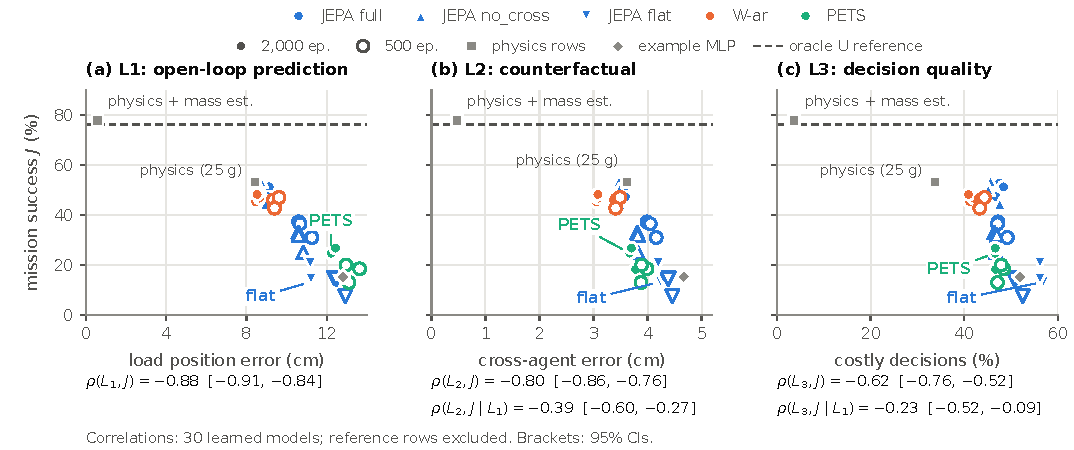
\includegraphics[width=\textwidth]{approved_figures_20261105/layers_vs_success.pdf}
\caption{Mission success against layers 1--3, one point per model. Open-loop error (left) tracks success most closely. PETS (green) has a larger open-loop error than JEPA \texttt{flat} (blue downward triangles) but a smaller cross-agent error (middle), and flies more often. Blue marks JEPA (circles \texttt{full}, upward triangles \texttt{no\_cross}) and orange W-ar; filled markers are for 2,000 training episodes, open for 500. Gray squares mark the physics rows and the gray diamond the example MLP; the dashed line is the oracle U. Each panel gives the Spearman correlation $\rho$ across the 30 learned models with its 95\% interval, and the middle and right panels also the partial correlation given layer~1,~\eqref{eq:partial}.}
\label{fig:scatter}
\end{figure*}

\section{Results}\label{sec:results}
% Budget: about 2 pages including Table II and Figs. 5-7. Narrated as World-in-World's Section 3: the benchmark,
% then the findings. Each paragraph opens with its claim in bold, gives one example in success rates or centimetres
% and at most one statistic, then its reading. Per-model numbers stay in Table II, how the episodes end in Fig. 6,
% and the correlations with their intervals in Figs. 5 and 7. Sources: uav_arena/README.md, "Results on test" and "Pre-registered analysis" (uav-arena 0fdb022),
% which print data/uav_arena/results/primary_analysis.json. Outside ANALYSIS.md, on the same 10,000 resamples:
% figures/src/rows_check.py (arena venv). Without PETS, rho(L2, J | L1) = +0.064 (-0.417 to +0.233); without flat,
% +0.195 (-0.164 to +0.288). PETS minus flat at 2,000 episodes, paired by seed: J +7.1 points (+2.8 to +12.2),
% L1 +1.33 cm (+0.86 to +1.78), L2 -0.53 cm (-0.58 to -0.48).

\subsection{Benchmark Results}
% README, "Results on test": U fails 95 of 400 episodes, 93 of them timeouts; physics + mass estimation against U,
% paired over layouts, +1.5 points (-3.0 to +6.0); nominal physics 53%, its most common failure a collision between
% aircraft (76 of 187), 41 of them on the ten layouts with 35.4-39.7 g loads, which pull the cables inward harder
% than the nominal model predicts ("Results on dev"). Learned rows at 2,000 episodes: full 50%, no_cross 49%, W-ar
% 47% (45% at 500); PETS and flat 12-23%; the best single model 54%; timeouts are 2-10% of their failures, obstacle
% collisions and collisions between aircraft 83-97%. CrazyMARL 41% (36-50% per seed), successes in 5.0 s against
% U's 7.5-8.2 s, every failure but one an obstacle collision, 2.1 s in on average; TD-MPC2 and DreamerV3 0 of 1,200.
\textbf{The reference rows set the scale, and the best learned world models fly about as often as nominal physics.} U predicts exactly, so its failures, nearly all of them timeouts, belong to the planner's search rather than to a model (Table~\ref{tab:results} and Fig.~\ref{fig:outcomes}). Physics with online mass estimation is level with U. With the nominal load mass, the same physics succeeds in about half of the missions, failing most often by collisions between aircraft, mostly on the heaviest loads, which pull the cables inward harder than it predicts. With all the training data, JEPA \texttt{full} and \texttt{no\_cross} and W-ar fly about as often as nominal physics, while PETS and \texttt{flat} succeed in at most one mission in four; unlike U, the learned rows fail mostly by collisions (Fig.~\ref{fig:outcomes}). Of the policies trained without the shared planner, CrazyMARL succeeds in about two missions out of five, and TD-MPC2 and DreamerV3 in none.

% Reference rows, example MLP and CrazyMARL: uav_arena/README.md, "Results on test" (uav-arena 7606aa0).
% Learned rows: the pooled table under "Pre-registered analysis" (uav-arena 0fdb022), J over the three seeds'
% 1,200 episodes with its interval, L1-L3 the mean of the three models. CrazyMARL's pooled interval, which the
% README does not give: figures/src/rows_check.py. Regenerate from the result files.
% TD-MPC2 and DreamerV3: test run of 2026-11-01; the README entry is still owed.
% Local review only. Same 17 result rows and original numerical values.
\begin{table}[t]
\caption{Benchmark Results Across Eight Test Conditions}
\label{tab:results}
\centering
\footnotesize
\setlength{\tabcolsep}{1.8pt}
\renewcommand{\arraystretch}{1.16}
\begin{tabular*}{\columnwidth}{@{\extracolsep{\fill}}lrrrrr@{}}
\hline
Method & \shortstack{Train\\ep.} & \shortstack{$J$ (\%) $\uparrow$\\{\scriptsize [95\% CI]}} & \shortstack{$L_1$\\(cm) $\downarrow$} & \shortstack{$L_2$\\(cm) $\downarrow$} & \shortstack{$L_3$\\(\%) $\downarrow$} \\
\hline
\multicolumn{6}{@{}l}{\rule{0pt}{2.1ex}\textbf{Reference rows, shared MPPI}} \\
U (oracle) & -- & 76.3 [65.0, 86.8] & 0 & 0 & 0 \\
Physics + mass est. & -- & 77.8 [67.5, 87.0] & 0.57 & 0.47 & 3.7 \\
Physics (25\,g) & -- & 53.3 [42.5, 64.3] & 8.42 & 3.62 & 33.8 \\
\hline
\multicolumn{6}{@{}l}{\rule{0pt}{2.1ex}\textbf{Learned world models, shared MPPI}} \\
Example MLP & -- & 15.3 [9.3, 22.3] & 12.81 & 4.67 & 51.9 \\
JEPA \texttt{full} & 500 & 34.9 [26.5, 43.6] & 10.84 & 4.07 & 47.8 \\
JEPA \texttt{full} & 2,000 & 50.4 [40.3, 60.3] & 9.01 & 3.56 & 47.6 \\
JEPA \texttt{no\_cross} & 500 & 30.0 [22.6, 37.8] & 10.67 & 3.82 & 46.7 \\
JEPA \texttt{no\_cross} & 2,000 & 49.4 [39.8, 59.0] & 8.80 & 3.48 & 46.1 \\
JEPA \texttt{flat} & 500 & 12.2 [7.1, 18.3] & 12.59 & 4.41 & 51.4 \\
JEPA \texttt{flat} & 2,000 & 16.2 [11.4, 21.5] & 11.20 & 4.25 & 56.4 \\
W-ar & 500 & 45.3 [36.2, 54.3] & 9.46 & 3.44 & 43.7 \\
W-ar & 2,000 & 46.8 [37.8, 55.5] & 8.55 & 3.07 & 41.4 \\
PETS & 500 & 17.2 [11.4, 23.7] & 13.24 & 3.92 & 47.8 \\
PETS & 2,000 & 23.3 [16.4, 30.9] & 12.53 & 3.72 & 46.6 \\
\hline
\multicolumn{6}{@{}l}{\rule{0pt}{2.1ex}\textbf{Policies without the shared planner}} \\
CrazyMARL & -- & 40.6 [30.0, 51.5] & -- & -- & -- \\
TD-MPC2 & -- & 0.0\textsuperscript{a} & -- & -- & -- \\
DreamerV3 & -- & 0.0\textsuperscript{a} & -- & -- & -- \\
\hline
\end{tabular*}
\par\vspace{2pt}
\begin{minipage}{\columnwidth}
\scriptsize\raggedright
400 test episodes per model. For three-seed methods, $J$ pools 1,200 episodes; $L_1$--$L_3$ are seed means. Brackets: 95\% bootstrap CIs over 50 layouts. Train ep.: offline training episodes; --: not reported or not applicable. \textsuperscript{a}Zero successes across all three seeds.
\end{minipage}
\end{table}

% Drawn by figures/src/plot_outcomes.py from the outcome counts of the test records (its docstring names the
% files). Success and timeout are neutrals; the failure types take categorical slots 4, 7 and 8, since slots 1-3
% name the model families in Figs. 1 and 5. About 2.75 in tall.
\begin{figure}[t]
\centering
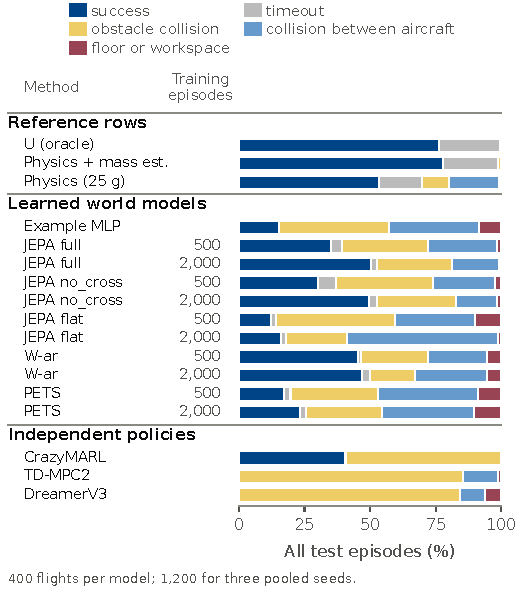
\includegraphics[width=\linewidth]{approved_figures_20261105/test_outcomes.pdf}
\caption{How the test episodes end, per row. Rows with three seeds pool their 1,200 episodes; the training-episodes column gives each world model's data budget. Nearly all of U's failures are timeouts; most of the learned models' and the policies' failures are collisions. Floor or workspace: an aircraft or the load hits the floor, or the team leaves the workspace.}
\label{fig:outcomes}
\end{figure}

\subsection{Findings}
% Finding 1: the primary test, decided by ANALYSIS.md, Section 4's rule; the between-row check is outside the plan
% (see the comment under the section heading). Finding 2 is its scope per condition (the README's table); findings 3
% and 4 are ANALYSIS.md, Section 5. Ordered on 2026-11-04 so that the claim and its scope come first.
% Fig. 7 (figures/src/plot_primary.py) draws the pooled test, the eight conditions and the between-row check.
\begin{figure}[t]
\centering
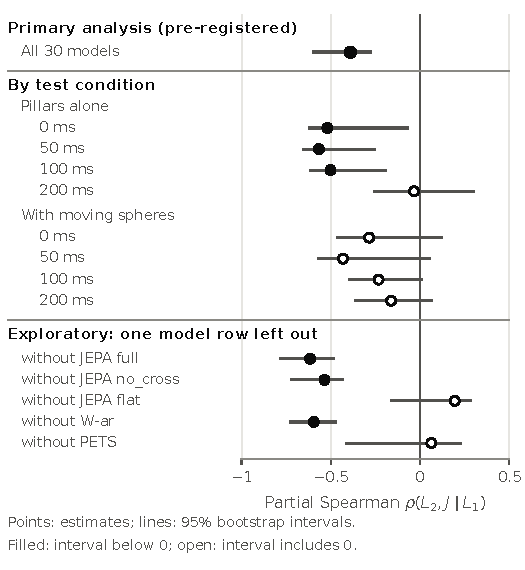
\includegraphics[width=\linewidth]{approved_figures_20261105/primary_statistic.pdf}
\caption{The partial Spearman correlation of layer~2 with success given layer~1,~\eqref{eq:partial}, with 95\% bootstrap intervals over layouts. Top: the pre-registered test across all 30 learned models. Middle: the eight test conditions. Bottom: an exploratory check outside the analysis plan, leaving out one model row's six models at a time. Filled markers indicate intervals entirely below zero; open markers indicate intervals containing zero.}
\label{fig:primary}
\end{figure}

\textbf{Cross-agent prediction explains success that open-loop prediction misses.} Open-loop error on U's plans is the best single guide to success (Fig.~\ref{fig:scatter}, left), but it misranks some models. PETS predicts the plans less accurately than JEPA \texttt{flat}, yet flies more often (23\% against 16\% at 2,000 episodes), and it predicts better how a change in one aircraft's plan spreads to the rest of the team (Fig.~\ref{fig:scatter}, middle). The pre-registered test asks whether, across the 30 models, cross-agent error explains success that open-loop error misses, and it does: once open-loop error is accounted for, higher cross-agent error goes with lower success, with a partial rank correlation of $-0.39$ (95\% interval $-0.60$ to $-0.27$), so the claim is supported. The evidence rests on these two rows: with either left out, a check outside the analysis plan, the interval contains zero (Fig.~\ref{fig:primary}). Open-loop error alone can therefore put a team's world models in the wrong order.

\textbf{Layer~2's contribution is clearest with the pillars alone and short delays.} Layer~2's partial correlation is negative in all eight conditions, but its interval lies below zero only with the pillars alone and delays up to 100\,ms (Fig.~\ref{fig:primary}). Layer~1 stays as closely tied to success in every condition as in the pooled test.

\textbf{Decision quality, the layer closest to the mission, tracks success least.} Every learned model makes costly decisions at roughly half of the questions, and the share follows success only loosely: with all the training data, PETS and JEPA \texttt{full} make costly decisions about equally often, yet \texttt{full} succeeds more than twice as often (Fig.~\ref{fig:scatter}, right). The partial correlation of layer~3 given layer~1 also lies below zero, but like layer~2's it rests on the PETS and \texttt{flat} rows. A likely reason is that the planner decides again 0.1\,s later, so one costly decision can be undone at the next, while the errors that end a mission compound on the states of the model's own flight, which only layer~4 sees.

% Structure and data size: README, "Pre-registered analysis". Entity tokens against flat: +28.5 and +25.5 points of
% J; four times the data: full +15.5, no_cross +19.4, flat +4.0 (0.0 to +7.7), W-ar +1.5 (-1.9 to +5.1), PETS +6.1;
% full against no_cross: J +3.0 points (0.3 to 5.8), L2 +0.16 cm. Collisions between aircraft at 2,000 episodes
% (Fig. 6): flat 691 of 1,200 episodes, full 214.
\textbf{Within JEPA, a token per aircraft matters, and direct attention between aircraft adds little.} The two variants with one token per aircraft and one for the load fly two and a half to three times as often as \texttt{flat}, which merges each frame into a single token, and predict cross-agent effects better (Table~\ref{tab:results}). With all the training data, more than half of \texttt{flat}'s missions end in a collision between aircraft, against fewer than one in five of \texttt{full}'s (Fig.~\ref{fig:outcomes}). Four times the data lifts these two variants from about a third to about half of the missions, while \texttt{flat}'s success does not change detectably. \texttt{no\_cross}, whose aircraft exchange information only through the load token, predicts cross-agent effects slightly better than \texttt{full} and succeeds slightly, but measurably, less often, so this pair runs against the primary relation. The simulator models no aerodynamic interaction between the aircraft: short of contact, they interact only through their cables and the load, the path that \texttt{no\_cross} keeps. More data lowers layers~1 and~2 for every row but raises success only for \texttt{full}, \texttt{no\_cross} and PETS; W-ar, like \texttt{flat}, succeeds about as often with a quarter of the data.


\section{Discussion}\label{sec:discussion}
% Budget, with the conclusion: about 0.75 page. The first paragraph draws the layers together: what each tells and
% what it misses (added 2026-11-04 so that the four layers argue rather than list). The rest, as in
% World-in-World's Section 4, each name an open problem in the first sentence; unlike it, also state the
% benchmark's own limits.

\textbf{What each layer tells.} Measured on the states the planner visits, open-loop error is the best single guide to whether a team's world model flies. It scores one plan, while the planner weighs many against one another, and layer~2, which asks how the predictions change when one aircraft's plan does, explains part of what it misses, here mainly the contrast between PETS and \texttt{flat}. Layer~3 scores single decisions at U's states; the next decision can undo a costly one, and the errors that end a mission compound along the model's own flight, which only layer~4 sees. Each layer thus answers a narrower question than mission success, and where two layers disagree, as for PETS and \texttt{flat}, the disagreement points to what a model gets wrong.

\textbf{\todo{The shared planner sets the ceiling.}} \todo{U fails 95 of 400 test episodes with exact predictions, so part of every row's failures belongs to the search, not the model; layers~2 and~3 separate the two. A stronger planner is future work, and so is an inference-compute axis (varying the MPPI sample budget), which the frozen analysis does not include.}

\textbf{\todo{Online model-based RL did not solve the task.}} \todo{TD-MPC2 and DreamerV3 succeeded in none of 2,400 test episodes; reported as is, outside the primary analysis.}

\textbf{\todo{From state to perception, and from simulation to flight.}} \todo{The arena observes states; onboard perception (cameras, for example) and real cables are open steps. One task, one planner and 30 models: say what generalizes and what does not. Layers~1--3 ask at U's states, and only layer~4 sees a model's own (Section~\ref{sec:fourlayers}); say more here only if space allows.}

\section{Conclusion}\label{sec:conclusion}
\todo{Three or four sentences: the question, the arena and its layers, the answer, and what it means for validating learned models before flight. Code and data availability.}

\section*{Acknowledgment}
\todo{Funding and acknowledgments, or delete this section.}

\bibliographystyle{IEEEtran}
\bibliography{references}

\end{document}
